\section*{Zadanie 16.}
\begin{task}
Narysować rozkład pól $E$ i $H$, wektora Poyntinga oraz prądów przewodzenia i przesunięcia w dwóch prostopadłych do siebie przekrojach wzdłużnych falowodu kołowego z falą A) bieżącą B) stojącą, rodzaju $E_{11}$. Opisać  jak będą się zmieniały te pola w funkcji czasu.\\
\end{task}

\begin{solution}

\begin{itemize}
	\item Fala bieżąca:
	\begin{center}
	$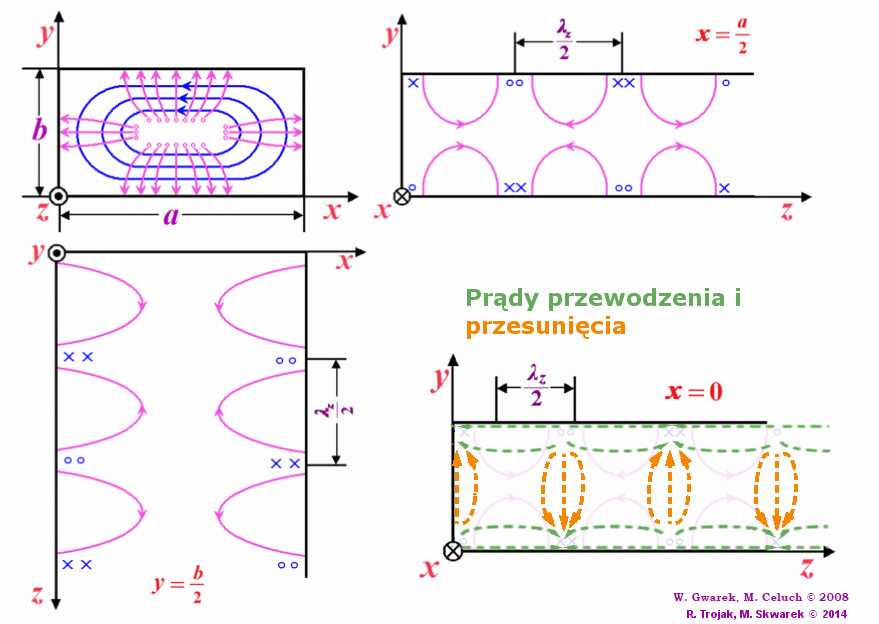
\includegraphics[scale=0.7]{16_1}$\\
	\end{center}
	\item Fala stojąca:\\
	
	
	\begin{center}
	$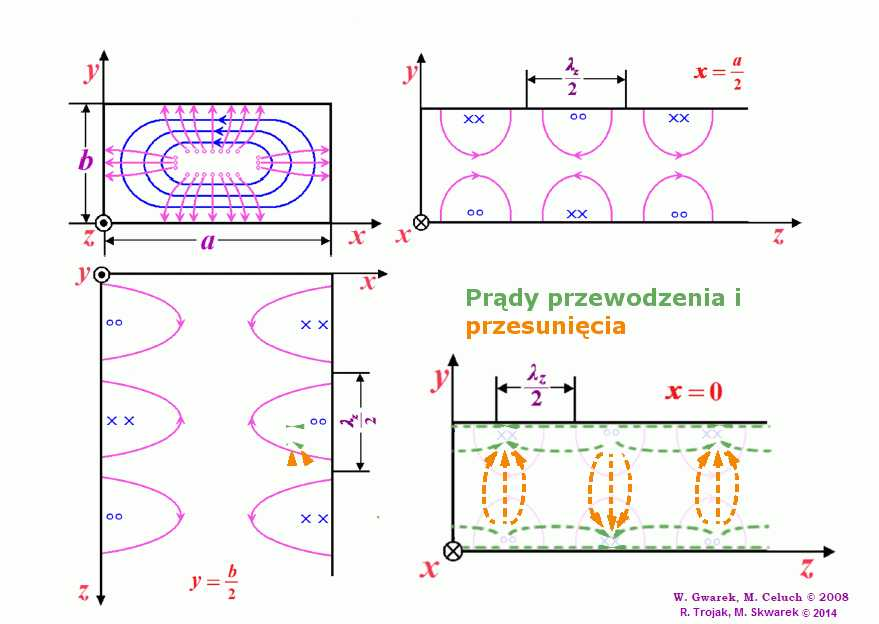
\includegraphics[scale=0.7]{16_2}$\\
	\end{center}
\end{itemize}
\end{solution}